\chapter{Аналитическая часть}

В данном разделе выполняется анализ предметной области хранения и обработки стоматологических снимков челюсти человека. Рассматриваются существующие программные решения, формализуются требования к разрабатываемой системе, выделяются основные категории хранимых данных и группы пользователей. Также проводится анализ моделей баз данных и обосновывается выбор реляционной модели данных.

\section{Анализ предметной области}

Стоматологическая диагностика включает сбор, хранение и анализ информации о состоянии зубочелюстной системы пациента. Одним из основных источников диагностической информации являются цифровые стоматологические снимки: панорамные снимки, прицельные снимки, телерентгенограммы и результаты компьютерной томографии. Такие изображения используются врачом для выявления патологий, планирования лечения, контроля динамики состояния пациента и документирования результатов медицинского обследования.

При работе со стоматологическими снимками необходимо хранить не только само изображение, но и набор связанных с ним данных: сведения о пациенте, дате загрузки снимка, типе исследования, оборудовании, на котором был получен снимок, медицинском специалисте, выполнившем анализ, и заключении врача. Такой подход соответствует общей практике хранения медицинских изображений, где важную роль играют как бинарные данные изображения, так и метаданные исследования~\cite{dicom-standard}.

В рамках рассматриваемой предметной области участвуют следующие основные категории пользователей:
\begin{itemize}
	\item врач-стоматолог --- анализирует снимки пациентов, формирует заключения и просматривает историю обследований;
	\item рентгенолог или лаборант --- загружает новые снимки, указывает тип исследования и оборудование;
	\item администратор --- управляет справочниками, клиниками, оборудованием и правами доступа.
\end{itemize}

Основная задача разрабатываемой системы заключается в централизованном хранении стоматологических снимков и связанных с ними медицинских данных. Система должна обеспечивать быстрый поиск снимков пациента, добавление новых исследований, создание врачебных заключений и управление справочной информацией.

\section{Анализ существующих решений}

В области хранения и обработки медицинских изображений существуют как универсальные, так и специализированные программные решения. К универсальным решениям относятся DICOM-серверы и PACS-системы, предназначенные для хранения медицинских изображений различных видов. К специализированным решениям относятся программные комплексы производителей стоматологического оборудования, ориентированные на работу с конкретными аппаратами и форматами данных.

В качестве примера специализированного решения можно выделить программное обеспечение Planmeca Romexis, предназначенное для работы со стоматологическими изображениями и данными пациентов~\cite{romexis}. Примером открытого решения для хранения медицинских изображений является Orthanc, представляющий собой легковесный DICOM-сервер~\cite{orthanc}.

Для сравнения существующих решений были выделены следующие критерии:
\begin{itemize}
	\item специализация на стоматологических снимках;
	\item возможность централизованного хранения изображений;
	\item гибкость ролевой модели доступа;
	\item возможность интеграции с собственной бизнес-логикой;
	\item стоимость внедрения и сопровождения;
	\item возможность использования внешнего кэширования.
\end{itemize}

Сравнение существующих решений приведено в таблице~\ref{tab:analogs}.

\begin{table}[H]
	\caption{Сравнение существующих решений}
	\label{tab:analogs}
	\centering
	\small
	\begin{tabular}{|p{0.25\textwidth}|p{0.18\textwidth}|p{0.18\textwidth}|p{0.25\textwidth}|}
		\hline
		Критерий & Planmeca Romexis & Orthanc & DentoBase \\
		\hline
		Специализация на стоматологии & да & нет & да \\
		\hline
		Централизованное хранение снимков & да & да & да \\
		\hline
		Гибкая ролевая модель & ограничена настройками продукта & требует настройки & проектируется на уровне БД \\
		\hline
		Возможность изменения бизнес-логики & ограничена & возможна через расширения & полная, так как система разрабатывается самостоятельно \\
		\hline
		Стоимость внедрения & высокая & низкая & низкая \\
		\hline
		Внешнее кэширование & зависит от конфигурации & требует отдельной настройки & проектируется как часть системы \\
		\hline
	\end{tabular}
\end{table}

Из таблицы видно, что существующие решения либо обладают избыточной функциональностью и высокой стоимостью, либо требуют дополнительной настройки для применения в стоматологической предметной области. Разрабатываемая система ориентирована на хранение и обработку именно стоматологических снимков и может быть адаптирована под требования конкретной клиники.

\section{Формализация задачи}

Необходимо разработать базу данных и приложение доступа к ней для хранения и обработки стоматологических снимков челюсти человека. Система должна обеспечивать хранение сведений о пациентах, врачах, лаборантах, клиниках, оборудовании, типах снимков, медицинских картах, снимках и врачебных заключениях.

В рамках поставленной цели необходимо решить следующие задачи:
\begin{itemize}
	\item проанализировать предметную область;
	\item определить основные сущности и связи между ними;
	\item сформулировать требования к базе данных и приложению;
	\item спроектировать реляционную базу данных;
	\item проверить соответствие базы данных третьей нормальной форме;
	\item спроектировать ролевую модель на уровне базы данных;
	\item спроектировать функции и триггеры на стороне базы данных;
	\item реализовать приложение доступа к базе данных;
	\item реализовать механизм внешнего кэширования с использованием Redis;
	\item провести тестирование разработанного приложения;
	\item исследовать влияние индексов на время выполнения запросов.
\end{itemize}

Разрабатываемая система должна поддерживать следующие основные варианты использования:
\begin{itemize}
	\item регистрация пациента;
	\item поиск пациента;
	\item создание медицинской карты;
	\item добавление нового стоматологического снимка;
	\item просмотр снимка;
	\item добавление врачебного заключения;
	\item управление справочниками;
	\item управление врачами, клиниками и оборудованием.
\end{itemize}

\section{Формализация данных}

На основании анализа предметной области были выделены следующие категории данных:
\begin{itemize}
	\item пациент;
	\item врач;
	\item клиника;
	\item лаборант;
	\item оборудование;
	\item тип снимка;
	\item стоматологический снимок;
	\item медицинская карта;
	\item диагноз или врачебное заключение;
	\item связь врача и клиники.
\end{itemize}

Сведения о категориях данных приведены в таблице~\ref{tab:data-categories}.

\begin{table}[H]
	\caption{Категории и сведения о данных}
	\label{tab:data-categories}
	\centering
	\small
	\begin{tabular}{|p{0.28\textwidth}|p{0.62\textwidth}|}
		\hline
		Категория & Сведения \\
		\hline
		Пациент & идентификатор, ФИО, дата рождения \\
		\hline
		Врач & идентификатор, специальность, список клиник, в которых работает врач \\
		\hline
		Клиника & идентификатор, адрес \\
		\hline
		Лаборант & идентификатор, ФИО, клиника работы \\
		\hline
		Оборудование & идентификатор, модель, клиника размещения \\
		\hline
		Тип снимка & идентификатор, название типа исследования \\
		\hline
		Снимок & идентификатор, бинарные данные изображения, дата загрузки, пациент, лаборант, оборудование, тип снимка \\
		\hline
		Медицинская карта & идентификатор, пациент, дата создания, дата обновления, признак активности, примечания \\
		\hline
		Диагноз & идентификатор, текст заключения, дата создания, снимок, врач, медицинская карта \\
		\hline
		Связь врача и клиники & идентификатор врача, идентификатор клиники \\
		\hline
	\end{tabular}
\end{table}

Между сущностями предметной области существуют следующие связи:
\begin{itemize}
	\item один пациент может иметь несколько снимков;
	\item один пациент может иметь несколько медицинских карт;
	\item одна медицинская карта может содержать несколько заключений;
	\item один снимок может иметь одно заключение;
	\item один врач может создать несколько заключений;
	\item одна клиника может иметь несколько единиц оборудования;
	\item одна клиника может иметь несколько лаборантов;
	\item один тип снимка может использоваться для нескольких снимков;
	\item один врач может работать в нескольких клиниках, и одна клиника может иметь нескольких врачей.
\end{itemize}

Последняя связь является связью многие-ко-многим. В дальнейшем она будет реализована с помощью ассоциативного отношения.

ER-диаграмма сущностей предметной области приведена на рисунке~\ref{fig:er-analytic}.

\begin{figure}[H]
	\centering
	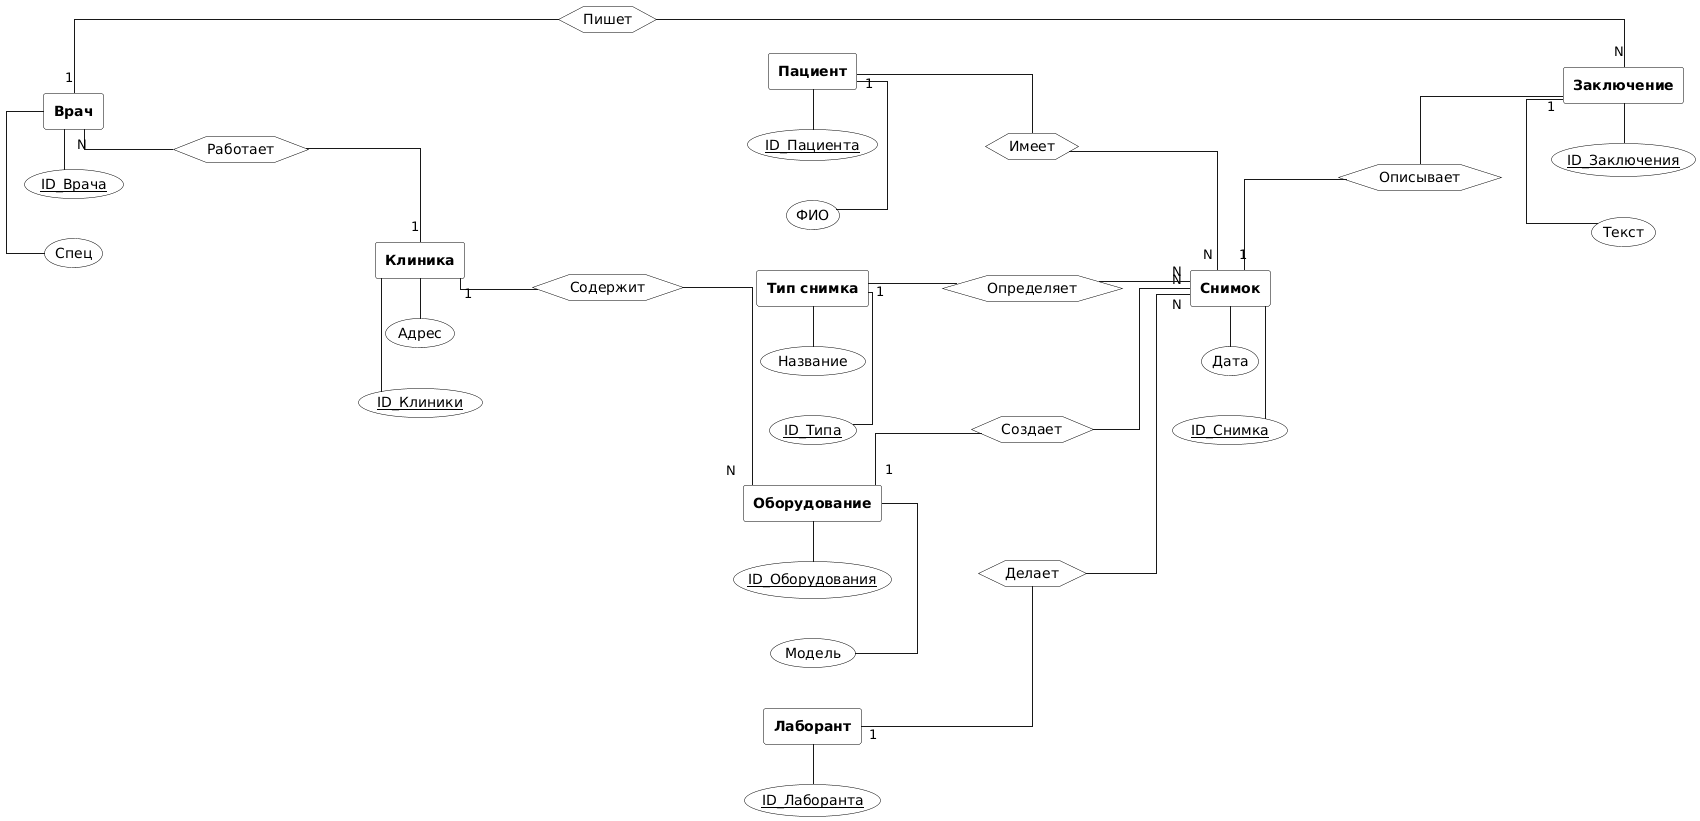
\includegraphics[width=\textwidth]{ER}
	\caption{ER-диаграмма сущностей предметной области}
	\label{fig:er-analytic}
\end{figure}

\section{Формализация пользователей}

В системе выделяются следующие группы пользователей:
\begin{itemize}
	\item врач-стоматолог;
	\item рентгенолог или лаборант;
	\item администратор.
\end{itemize}

Врач-стоматолог просматривает данные пациентов, изучает снимки и формирует медицинские заключения. Рентгенолог загружает снимки и указывает сведения об исследовании. Администратор управляет справочниками, клиниками, оборудованием, пользователями и правами доступа.

Описание ролей пользователей приведено в таблице~\ref{tab:user-roles}.

\begin{table}[H]
	\caption{Пользователи системы}
	\label{tab:user-roles}
	\centering
	\small
	\begin{tabular}{|p{0.28\textwidth}|p{0.62\textwidth}|}
		\hline
		Пользователь & Действия \\
		\hline
		Врач-стоматолог & поиск пациента, просмотр снимков, просмотр медицинской карты, добавление заключения \\
		\hline
		Рентгенолог & регистрация пациента, загрузка снимка, выбор типа снимка и оборудования \\
		\hline
		Администратор & управление справочниками, клиниками, врачами, оборудованием и правами доступа \\
		\hline
	\end{tabular}
\end{table}

Диаграмма вариантов использования приведена на рисунке~\ref{fig:use-case}.

\begin{figure}[H]
	\centering
	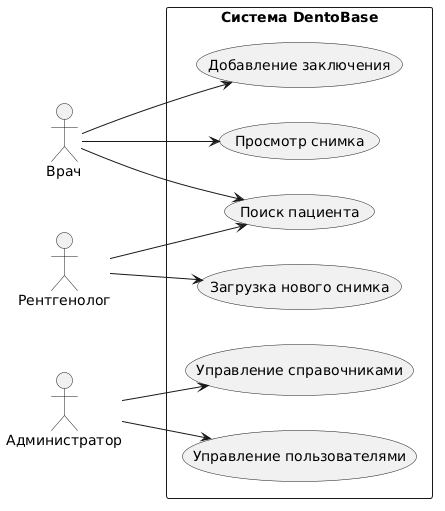
\includegraphics[width=0.7\textwidth]{use-case}
	\caption{Диаграмма вариантов использования}
	\label{fig:use-case}
\end{figure}

\section{Анализ моделей баз данных}

База данных представляет собой организованную совокупность данных, предназначенную для долговременного хранения и использования прикладными программами~\cite{date-db}. Система управления базами данных обеспечивает создание, изменение, поиск, защиту и поддержание целостности данных~\cite{silberschatz-db}.

По модели организации данных можно выделить следующие основные типы баз данных:
\begin{itemize}
	\item иерархические;
	\item сетевые;
	\item реляционные;
	\item объектно-реляционные;
	\item документоориентированные.
\end{itemize}

Иерархическая модель представляет данные в виде дерева. Такая модель удобна для описания строго иерархичных структур, однако плохо подходит для предметной области, где между сущностями существует большое количество связей разных типов.

Сетевая модель позволяет описывать более сложные связи между данными, чем иерархическая, однако требует более сложной навигации между записями и теснее связывает прикладную логику со структурой хранения данных.

Документоориентированная модель удобна для хранения слабоструктурированных данных, но в рассматриваемой задаче важную роль играют строгие связи между пациентами, снимками, врачами, клиниками и медицинскими картами. Для таких данных требуется контроль ссылочной целостности.

Реляционная модель представляет данные в виде отношений, то есть таблиц, и позволяет задавать первичные ключи, внешние ключи и ограничения целостности~\cite{date-db,postgresql-constraints}. В рассматриваемой системе данные имеют четкую структуру, а связи между сущностями заранее известны. Поэтому реляционная модель является наиболее подходящей.

Для реализации базы данных выбрана PostgreSQL. Данная СУБД поддерживает реляционную модель данных, транзакции, индексы, ограничения целостности, роли, функции и триггеры~\cite{postgresql-docs,postgresql-triggers,postgresql-privileges}. Эти возможности необходимы для выполнения требований к разрабатываемой системе.

\section*{Вывод}
\addcontentsline{toc}{section}{Вывод}

В аналитической части была рассмотрена предметная область хранения и обработки стоматологических снимков челюсти человека. Были проанализированы существующие решения, сформулирована задача, выделены основные категории данных и пользователи системы. Также были рассмотрены модели баз данных и обоснован выбор реляционной модели данных и PostgreSQL в качестве СУБД.

\clearpage